\section{Methodology}
\label{sec}

\subsection{Data Collection}
\label{subsec:data_collection}
The dataset used in this research is based on the ITC2007 Track 3: Curriculum-Based Course Timetabling (CB-CTT). This dataset has instances where it contains detailed information. This information include a header and four main sections: courses, rooms, curricula, and constraints, with each section containing arrays corresponding to a specific component in the problem and all scalar values summarised in the header. Each dataset instance provides the basic information for testing and validating the proposed approach. 

\begin{figure}[] % h stands for 'here'
    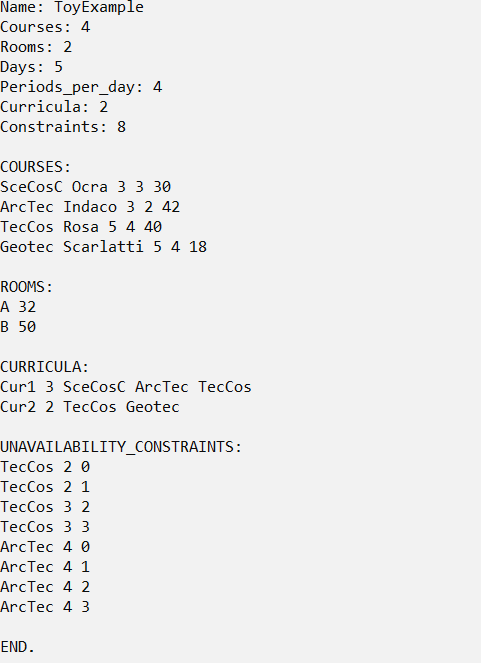
\includegraphics[width=1\textwidth]{example.png}
    \caption{Example of CB-CTT Instance}
    \label{fig:example} % label for referencing
\end{figure}

\clearpage

The header describes the important properties of the instance: name of the instance, number of courses, rooms, working days, periods per day, curricula, and constraints. These values determine the scope and size of the timetabling problem and the boundaries of feasible scheduling.

In the \textbf{Courses} section, every course is specified to include the assigned teacher, number of lectures required, minimum number of working days that lectures should be spread, and number of students enrolled. 

The \textbf{Rooms} section defines the rooms available for scheduling along with their seating capacities. 

Under \textbf{Curricula}, the courses of similar curricula are combined together such that no two classes from a particular curriculum fall at the same time. 


The \textbf{Unavailability Constraints} section specifies day-period combinations during which certain courses cannot be scheduled. These constraints typically arise from limitations such as teacher unavailability or room restrictions. 

This structured dataset gives a stable base for testing and verification of the proposed MSPSO, thus ensuring that all the constraints imposed on it are well described.

\subsection{Data Processing}
\label{subsec:data_processing}

The data processing phase transforms the raw dataset into a structured and optimized format suitable for integration into the MSPSO framework. All problem components and constraints are accurately represented to allow seamless initialization of particles and candidate solution evaluation.

The dataset contains courses, rooms, curricula, and unavailability constraints, which are parsed and normalized in order to achieve consistency. Time-related data, that is, days and periods, are converted to numerical indices, and the constraints are encoded to lead the process of optimization. The parsed data is structured into a particle representation, that is, encoding each candidate solution of the timetabling problem as a list of scheduling entries in the format:

\[
(\text{Day}, \text{Period}, \text{Room}, \text{Course}).
\]

\subsubsection*{Constraint Encoding}

The constraints, central to the problem, can be categorized into two types, namely hard constraints and soft constraints. Hard constraints are mandatory and must be strictly satisfied, while soft constraints are desirable properties that contribute to the overall quality of the solution. The details and mathematical representations of these constraints are given as follows:

\clearpage

\begin{table}[h]
    \centering
    \begin{tabular}{|c|p{10cm}|}
    \hline
    \textbf{Symbol} & \textbf{Definition} \\ \hline
    \(d, p, r, c\) & Day, Period, Room, and Course respectively. \\ \hline
    \(S\) & Set of all scheduling entries, where each entry is \((d, p, r, c)\). \\ \hline
    \(U\) & Set of unavailability constraints, specifying unavailable periods for certain courses. \\ \hline
    \(\operatorname{Curr}(k)\) & Set of courses in curriculum \(k\). \\ \hline
    \(T(c)\) & Teacher assigned to course \(c\). \\ \hline
    \(\text{students}(c)\) & Number of students enrolled in course \(c\). \\ \hline
    \(\text{capacity}(r)\) & Capacity of room \(r\). \\ \hline
    \(\text{min\_days}(c)\) & Minimum number of days required for course \(c\). \\ \hline
    \(R_c\) & Set of rooms assigned to course \(c\) across all scheduled periods. \\ \hline
    \end{tabular}
    \caption{Symbols used for the CB-CTT problem}
    \label{tab:symbols}
\end{table}

\paragraph*{Hard Constraints}

\begin{enumerate}
    \item \textbf{Lecture Assignment}:
    Each lecture of a course must be assigned to a unique combination of day, period, and room. Overlaps are strictly prohibited.
    \[
    \forall (d, p, r, c_i), (d', p', r', c_j) \in S, \quad i \neq j \Rightarrow (d, p, r) \neq (d', p', r').
    \]

    \item \textbf{Room Occupancy}:
    No two lectures can occupy the same room at the same time.
    \[
    \forall (d, p, r, c_i), (d, p, r, c_j) \in S, \quad i \neq j \Rightarrow c_i \neq c_j.
    \]

    \item \textbf{Conflicts}:
    Courses in the same curriculum or taught by the same teacher must not overlap in time.
    \[
    \forall (d, p, r, c_i), (d, p, r', c_j) \in S, \quad (c_i \in \operatorname{Curr}(k) \lor T(c_i) = T(c_j)) \Rightarrow p_i \neq p_j.
    \]
    Here, \(\operatorname{Curr}(k)\) represents the courses in curriculum \(k\), and \(T(c)\) is the teacher assigned to course \(c\).

    \item \textbf{Availability}:
    Courses cannot be scheduled during unavailable periods as specified in the dataset.
    \[
    \forall (c, d, p) \in U, \quad (d', p', r, c') \in S, \quad c' = c \Rightarrow (d' \neq d \lor p' \neq p).
    \]
\end{enumerate}

\paragraph*{Soft Constraints}

\begin{enumerate}
    \item \textbf{Room Capacity}:
    Assigning a course to a room with insufficient capacity incurs a penalty proportional to the seating deficit.
    \[
    P_1 = \sum_{(d, p, r, c) \in S} \max(0, \operatorname{students}(c) - \operatorname{capacity}(r)).
    \]

    \item \textbf{Minimum Working Days}:
    Scheduling a course for fewer days than its minimum requirement results in a penalty.
    \[
    P_2 = \sum_{c \in C} 5 \cdot \max(0, \operatorname{min\_days}(c) - |\{d \mid (d, p, r, c) \in S\}|).
    \]

    \item \textbf{Room Stability}:
    Assigning a course to multiple rooms across its schedule incurs a penalty for each additional room used.
    \[
    P_3 = \sum_{c \in C} \max(0, |R_c| - 1), \quad R_c = \{r \mid (d, p, r, c) \in S\}.
    \]

    \item \textbf{Curriculum Compactness}:
    Isolated lectures for a curriculum within a day are penalized, promoting schedule compactness.
    \[
    P_4 = \sum_{k} \sum_{d} \sum_{p \in P_d} \operatorname{is\_isolated}(p),
    \]
    where \(\operatorname{is\_isolated}(p) = 2\) if no adjacent lectures exist for curriculum \(k\).
\end{enumerate}

\subsubsection*{Fitness Function}

The overall fitness function integrates the penalties for soft constraints and serves as the objective function for optimization. It is expressed as:
\[
\text{Fitness} = Penalty = P_1 + P_2 + P_3 + P_4.
\]

\subsubsection*{Validation and Testing}

The parsed data is verified for completeness and consistency during the process. It checks to ensure that all courses, rooms, and curricula have been represented accurately and the constraints are correctly encoded. Thus, the structured and validated data forms a robust base for initializing particles and guiding the optimization process.

The approach of comprehensive data processing will prepare the problem constraints and components for the MSPSO framework in an accurate manner so that hard constraints are maintained and soft constraint penalties are optimized.

\subsection{Approach Construction}
\label{subsec:approach_construction}

The approach begins with initializing particles in the Multi-Swarm Particle Swarm Optimization (MSPSO) algorithm. Each particle represents a potential solution—a timetabling configuration. 

\begin{algorithm}[H]
    \small
    \caption{Multi-Swarm Particle Swarm Optimization Algorithm}
    \begin{algorithmic}[1]
    \State Initialize swarms, particles, and parameters
    \For{each iteration up to \texttt{max\_iterations}}
        \State Compute convergence and exclusion radius $r_\text{rconv} $ $r_\text{excl}$
        \State \textit{// Anti-Convergence}
        \If{all swarms converged and swarm limit not exceeded}
            \State Add new swarm with random initialization
        \EndIf 

        \If{all swarms converged}
            \State Randomize worst-performing swarm
        \EndIf

        \State \textit{// Exclusion}
        \For{each pair of swarms in the population}
            \State Compute distance between best particles of swarms
            \If{distance $<$ \texttt{rexcl}}
                \State Reinitialize the worse swarm
            \EndIf
        \EndFor

        \State \textit{// Update and Randomize Particles:}
        \For{each swarm in the population}
            \If{swarm needs reinitialization}
                \State Reinitialize particles using quantum reinitialization
            \Else
            \For{each particle $p$ in swarm}
                \State Update position using move and swap
                \State Evaluate fitness and update personal/local bests
            \EndFor
            \EndIf
        \EndFor
        \State \textit{// Global Best Update}
        \If{better global fitness found}
            \State Update global best particle
        \EndIf
        
        \If{global best fitness $\leq$ target}
            \State \textbf{Break}
        \EndIf
    \EndFor
\end{algorithmic}
\end{algorithm}
    
\subsubsection{Initialization Phase}
\label{subsubsec:initialization}

In the initialization phase, initial solutions (particles) and swarms are generated to represent potential timetables for the Curriculu-Based Course Timetabling Problem (CBCTT). A graph heuristic approach \cite{mohamed2020constructing} is used to ensure the creation of feasible and efficient initial particles. Specifically, the Largest Degree (LD) heuristic is applied to determine the sequence of courses to be scheduled. Courses with the most unavailability constraints, constraints given in the input, are prioritized for assignment.

Once the sequence of courses is computed by the LD heuristic, an assignment of all the lectures that haven't been assigned yet to definite time slots and rooms is undertaken. This step is done in a systematic procedure for it to remain feasible and valid under the constraint. A cycle of procedures can be applied, each of them addressing different potential scenarios:
    
\begin{itemize}
    \item[] \textbf{Random Assignment (Procedure 1):}  

    Each unassigned course is assigned to an available and empty slot that fulfills all constraints such as room capacity or availability. For instance, in this procedure, Lecture 1 is initially unassigned. The system recognizes Room 1 in Slot i as an available and empty slot that meets all conditions such as room capacity or availability. Lecture 1 is then assigned to this room. In the picture, initially, the room, Room 1, is marked as (Empty) with a yellow fill, though it is available for Lecture 1. After the assignment, Room 1 is highlighted in orange; Lecture 1 was assigned to it without conflict.

    \begin{figure}[H]
        \centering
        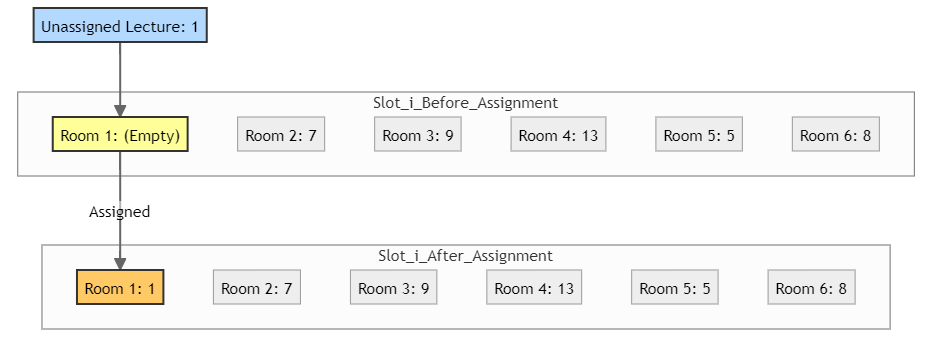
\includegraphics[width=1\textwidth]{procedure1_random_assignment.png}
        \caption{Procedure 1: Random Assignment - Before and After}
        \label{fig:random_assignment}
    \end{figure}

    \item[] \textbf{Conflict-Resolution Assignment (Procedure 2):}  
    
    If no empty slot is available, the lectures are placed in slots with minor conflicts. The conflicting lecture in the selected slot is then reallocated to another valid slot to remove conflict and maintain feasibility. For instance, in this procedure, Lecture 1 is unassigned and needs to be scheduled. Room 4 in Slot i is the best slot, but it is occupied by Lecture 13. Lecture 13 is moved to Room 3 in Slot j, which is free and satisfies all the constraints. After resolving the conflict, Lecture 1 is assigned to Room 4 in Slot i. In the example, to illustrate before the assignment, Room 4 is colored red, which shows that it has a clash with Lecture 1. Room 3 in Slot j is colored blue, indicating that it is free to hold Lecture 13. After resolving the conflict, Lecture 1 was properly assigned to Room 4, now showing the color orange.

    \begin{figure}[H]
        \centering
        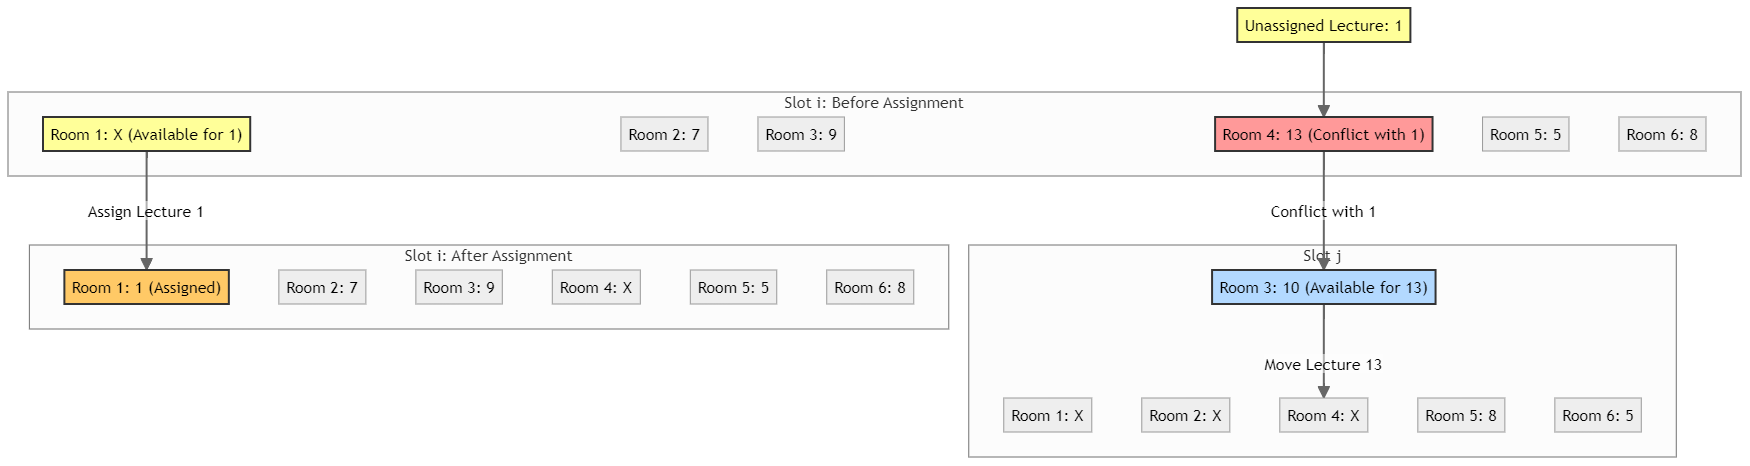
\includegraphics[width=1\textwidth]{procedure2_conflict_resolution.png}
        \caption{Procedure 2: Conflict Resolution - Before and After}
        \label{fig:conflict_resolution}
    \end{figure}

    \item[] \textbf{Swappable Slot Assignment (Procedure 3):}  
    
    If there are no empty slots available, the lecture is assigned to a slot that has minor conflicts, and the conflicting lecture is reassigned. For instance, in this algorithm, Lecture 1 is left unassigned and there is no empty slot in Slot i. However, Room 4 is identified as a swappable slot because it contains Lecture 6, which can be swapped without violating any constraints. The system switches the lectures by moving Lecture 6 to Room 3 in Slot j which is free, so that makes room 4 free in slot i, therefore lecture 1 is assigned in that room. In the example, Room 4 is colored yellow to show it is a good fit for Lecture 1. Room 3 in Slot j is colored blue as available for Lecture 6. After the exchange, Lecture 1 is placed in Room 4 and is colored orange. Lecture 6 is successfully switched to Room 3 in Slot j.


    \begin{figure}[H]
        \centering
        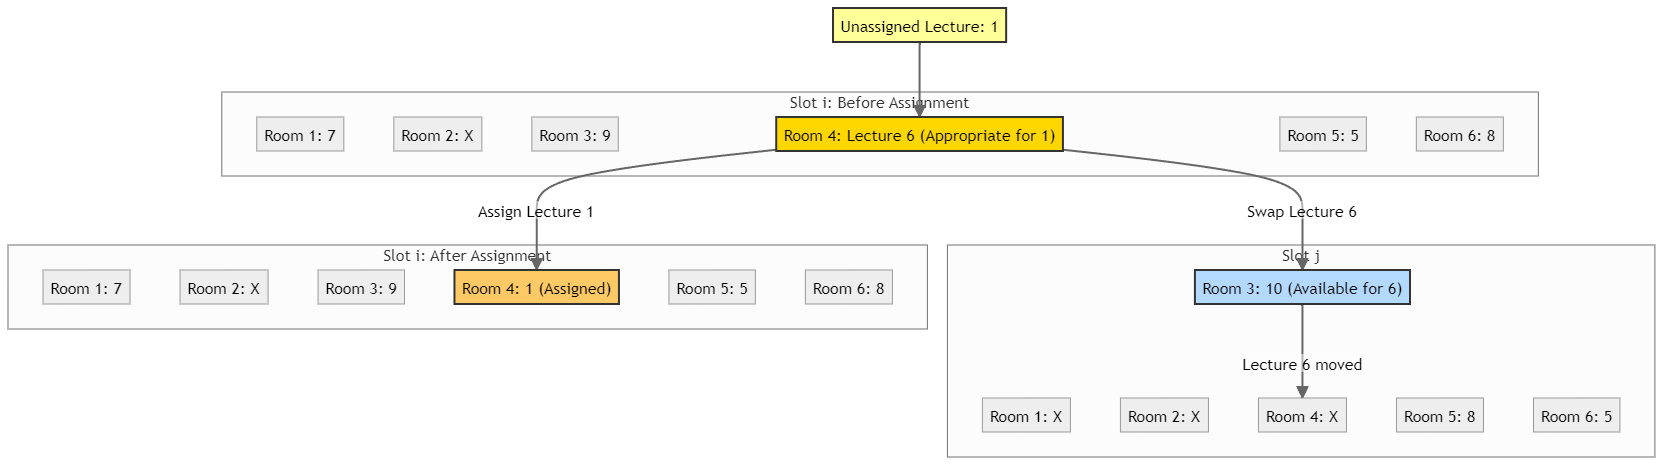
\includegraphics[width=1\textwidth]{procedure3_swappable_slot.png}
        \caption{Procedure 3: Swappable Slot Assignment - Before and After}
        \label{fig:swappable_slot}
    \end{figure}

    \item[] \textbf{Override Assignment (Procedure 4):}  
    
    If no others are available a conflicting slot overrides all lectures and is scheduled In this procedure: Lecture 1 is unassigned and all such slots are utilized. The system finds Room 3 in Slot i as the most appropriate slot but finds Lecture 8 in the same room. It overwrites the conflict by moving Lecture 8 to Room 2 in Slot j, which is free and satisfies all constraints. Once the conflict is resolved, it assigns Lecture 1 to Room 3 in Slot i. In the figure, Room 3 is colored red to indicate that it conflicts with Lecture 1, and Room 2 in Slot j is colored blue to indicate that it is available for Lecture 8. After resolution, Lecture 1 is assigned to Room 3, now colored orange, and Lecture 8 is successfully moved to Room 2 in Slot j.

    \begin{figure}[H]
        \centering
        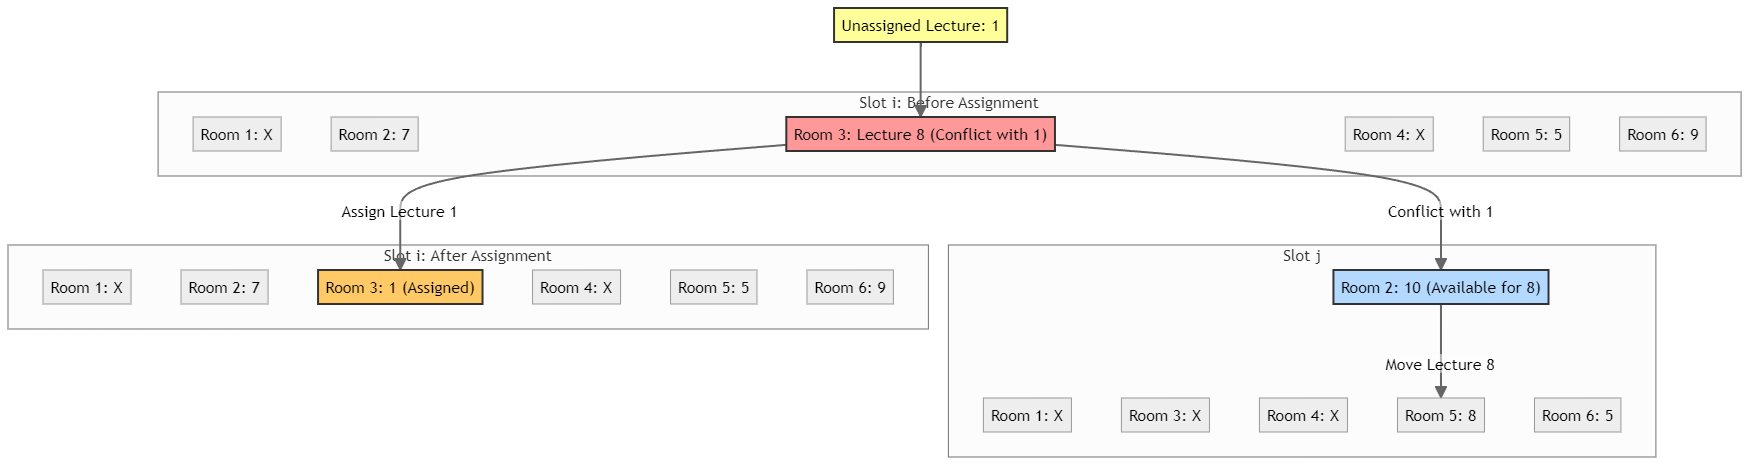
\includegraphics[width=1\textwidth]{procedure4_override_assignment.png}
        \caption{Procedure 4: Override Assignment - Before and After}
        \label{fig:override_assignment}
    \end{figure}

\end{itemize}

After the first timetable is created, it is expressed as a set of schedule entries, with each entry containing day, period, room, and course. The initial population of the optimization process is represented by these timetables and is further partitioned into swarms that will be used for further exploration and refinement in the subsequent phases.

\begin{figure}[H]
    \centering
    
\includegraphics[width=1\textwidth]{timetable_particles.png} 
    \caption{Particle as timetable entries}
    \label{fig:timetable_particles}
\end{figure}\subsubsection{Optimization Phase}
\label{subsubsec:optimization}

The MSPSO algorithm refines the initial solutions generated by the graph-based heuristic through a series of systematic optimization steps. The optimization loop includes the initialization of critical parameters, anti-convergence checks, exclusion mechanisms, particle updates and reinitialization, and global best updates. Each of these components plays a crucial role in iteratively improving the solutions to minimize penalties and adhere to hard and soft constraints.

\paragraph{Initialization of Parameters}
Before the optimization begins, several parameters are initialized:

\begin{itemize}
    \item \textbf{Swarm and Particle Structure:} Each swarm contains several particles, where every particle is a candidate solution, and the form it represents is a feasible schedule. The feasible schedules are encoded as lists of assignments, and every assignment describes a solution as \textit{day}, \textit{period}, \textit{room\_id}, and \textit{course\_id}respectively. Every particle further contains such features as its fitness value, velocity, and best solutions found by it in the process of optimization. This swarm structure enables particles to interact and exchange information for better results.
    
    \item \textbf{Global and Local Parameters:} Key parameters are defined to guide the behavior of the algorithm. Table~\ref{tab:global_local_parameters} provides an overview of the parameters and their corresponding values used in this research.

    \begin{table}[H]
        \centering
        \renewcommand{\arraystretch}{1.5} % Adjust row height
        \begin{tabularx}{\textwidth}{|p{3cm}|p{2cm}|>{\raggedright\arraybackslash}X|}
            \hline
            \textbf{Parameter} & \textbf{Value} & \textbf{Description} \\ \hline
            \texttt{NPARTICLES} & 5 & Number of particles in each swarm, representing candidate solutions. \\ \hline
            \texttt{NSWARMS} & 1 & Number of swarms initialized for parallel exploration of the solution space. \\ \hline
            \(\chi\) (Inertia) & 0.729 & Controls the influence of a particle's previous velocity in the current update. \\ \hline
            \(c_1\) (Personal Best Coefficient) & 1.0 & Determines the influence of a particle's personal best position on the velocity update. \\ \hline
            \(c_2\) (Global Best Coefficient) & 1.0 & Determines the influence of the global best position on the velocity update. \\ \hline
            \texttt{rexcl} & Dynamic (Based on iteration) & Define the exclusion radius so that the swarms start exploring different areas of the solution space. Given by \( \texttt{rexcl} = (\texttt{BOUNDS} / \texttt{NSWARMS})^{1 / \texttt{NDIM}} \). \\ \hline
            \texttt{rconv} & Same as \texttt{rexcl} & It denotes the convergence radius in the anti-convergence. This prevents the swarms from premature convergence mechanism by keeping a minimum distance between the particles in the swarm. Given by \( \texttt{rconv} = \texttt{rexcl} \) \\ \hline
            \texttt{RCLOUD} & 0.5 & Defines the radius for quantum reinitialization around the global best to introduce diversity. \\ \hline
        \end{tabularx}
        \caption{Global and Local Parameters for MSPSO}
        \label{tab:global_local_parameters}
    \end{table}
    

\begin{itemize}
    \item \textit{Number of Particles and Swarms (\texttt{NPARTICLES} and \texttt{NSWARMS}):} These represent the number of particles and swarms, which decide the initial population size and the degree of parallel exploration of the optimization algorithm. Each particle is a candidate solution, and the swarms operate in parallel to increase the diversity.
    
    \item \textit{Coefficients (\(\chi\), \(c_1\), \(c_2\)):} The coefficients are critical to the balance of exploration and exploitation:
    \begin{itemize}
        \item \(\chi\) controls the inertia or the influence of a particle's previous velocity on its current update.
        \item \(c_1\) modifies the attraction towards a particle's personal best solution.
        \item \(c_2\) modifies the attraction toward the local best solution found by the swarm.
    \end{itemize}
    \item \textit{Radius Parameters (\texttt{rexcl}, \texttt{RCLOUD}, and \texttt{rconv}):} These parameters define key distance measures:
    \begin{itemize}
        \item \texttt{rexcl} ensures that swarms remain diverse by preventing convergence to the same solution area. It is dynamically calculated based on the bounds and dimensionality of the search space.
    
        \( \texttt{rexcl} = (\texttt{BOUNDS} / \texttt{NSWARMS})^{1 / \texttt{NDIM}} \)

        \item \texttt{RCLOUD} defines the radius for quantum-inspired reinitialization around the global best, helping to reintroduce diversity when swarms converge prematurely.
        \item \texttt{rconv} is used in the anti-convergence mechanism, representing the convergence radius. It ensures that particles maintain a minimum distance from one another, thereby avoiding premature convergence and ensuring better exploration of the solution space.
    \end{itemize}
\end{itemize}

    \item \textbf{Fitness Evaluation:} The initial fitness of each particle is calculated based on penalties for violations of soft constraints. Such penalties include room capacity overuse, insufficient minimum days for lectures, lack of room stability, and issues of compactness in the curriculum. The total penalty represents the quality of the schedule, and the lower values are indicative of better solutions.
    
    \[
    \text{Penalty} = P_1 + P_2 + P_3 + P_4
    \]
    where:
    \begin{itemize}
        \item $P_1$: Penalty for room capacity, 
        \item $P_2$: Penalty for minimum working days
        \item $P_3$: Penalty for room stability
        \item $P_4$: Penalty for curriculum compactness
    \end{itemize}

\end{itemize}

\paragraph{Anti-Convergence Check}\

The anti-convergence check \cite{Blackwell2006-ms} makes sure that the optimization process avoids stagnation in the exploration of the solution space and maintains diversity. This mechanism checks whether all particles in a swarm have converged too closely and are not able to explore new regions.

The reinitialization radius (\texttt{rconv}) is an important parameter in the anti-convergence process. It controls the movements of particles during reinitialization so that diversity is injected into the swarm. It is calculated as:

\[
\texttt{rconv} = \frac{\texttt{BOUNDS}}{\texttt{len(population)}^{(1.0 / \texttt{NDIM})}}
\]

where \(\texttt{BOUNDS}\) is the size of the solution space, \(\texttt{len(population)}\) is the current number of swarms, and \(\texttt{NDIM}\) is the number of problem dimensions. Then, define a threshold to detect convergence as the diameter of the convergence sphere as \(2 \times \texttt{rconv}\). If all distances between particles are smaller than \(2 \times \texttt{rconv}\), then the swarm is considered converged. Thus, using the diameter as a threshold marks effective identification of tightly clustered particles, hence swarm reinitialization and stagnation prevention.

Pairwise Euclidean distances \cite{ClusterAnalysis2023} between particles are computed using normalized dimensions for \textit{day}, \textit{period}, and \textit{room}. The calculation accounts for the total number of days, periods, and rooms to ensure proper scaling. The formula for distance (\(d\)) is given as:

\[
d = \sqrt{
\sum \left( 
\frac{(\text{day}_{p1} - \text{day}_{p2})}{\text{total days}}^2 +
\frac{(\text{period}_{p1} - \text{period}_{p2})}{\text{total periods}}^2 +
\frac{(\text{room}_{p1} - \text{room}_{p2})}{\text{total rooms}}^2 
\right)
}
\]

where \(p1\) and \(p2\) represent particles in the swarm. If all distances between particles are less than the convergence threshold (\(2 \times \texttt{rconv}\)), the swarm is deemed converged. Using (\(2 \times \texttt{rconv}\)) as threshold is based on the fact that doubling the radius gives the diameter, which shows the maximum permissible distance between two particles in any swarm. For all distances falling below this threshold, it depicts that the swarms are so tightly clustered to confirm convergence; hence, using this method makes it possible for converged swarms to be further reinitialized towards better coverage of the search space and less stagnation during the process.

For this reason, reinitialization can be triggered every time a swarm is converged heavily and its swarm's best fitness is one of the worst found in the population. The introduction of diversity results from the swapping process, as this reinitialization procedure makes way for particles that can move the swarm around regions it has not seen before, further away from possible local optima.

If all swarms have converged and the total number of swarms is still less than the maximum allowed number (defined as \texttt{NSWARMS} + \texttt{NEXCESS}), more swarms are initialized. New swarms will begin with randomly assigned particle positions to enhance exploration in the optimization process. This means that the search algorithm will not be degraded, even in a very challenging landscape, and should find optimal solutions.

The success of this mechanism depends highly on the reinitialization radius, \texttt{rconv}, which is a key factor in the anti-convergence process. The \texttt{rconv} parameter controls the movement of particles in the reinitialization process so that diversity is injected back into the swarm. With a controlled radius for particle reinitialization, \texttt{rconv} prevents convergence in a swarm and allows for the exploration of new regions in the solution space. This focused approach makes sure that the algorithm stays dynamic and can always find better solutions by avoiding stagnation and local optima.

\paragraph{Exclusion Mechanism}\

The exclusion mechanism ensures that different swarms explore distinct regions of the solution space, preventing convergence to similar solutions. This mechanism calculates the pairwise distances between the best particles of every pair of swarms using a normalized Euclidean distance formula. The distance is computed as follows:

\[
\text{distance} = \sqrt{
\sum \left(
\frac{(\text{day}_{p1} - \text{day}_{p2})}{\text{total days}}^2 +
\frac{(\text{period}_{p1} - \text{period}_{p2})}{\text{total periods}}^2 +
\frac{(\text{room}_{p1} - \text{room}_{p2})}{\text{total rooms}}^2
\right)
}
\]

where \(p1\) and \(p2\) are the best particles from two different swarms. If the computed distance is less than the exclusion radius (\(\texttt{rexcl}\)), the swarm with the worse fitness among the two is reinitialized. The exclusion radius is dynamically determined as:

\[
\texttt{rexcl} = \texttt{rconv}
\]

\paragraph{Quantum Reinitialization}\

Quantum reinitialization ensures that diversity is injected back into the swarm when it shows signs of premature convergence. This forms new particle positions using a Gaussian perturbation about the global best particle. This is shown in Algorithm \ref{alg:quantum_reinit}.

\begin{algorithm}[H]
    \caption{Quantum Reinitialization}
    \label{alg:quantum_reinit}
    \begin{algorithmic}[1]
        \For{each particle $p$ in the swarm}
            \If{$p$ is the global best}
                \State Skip reinitialization
            \Else
                \For{each assignment in $p$}
                    \State Generate $new\_day$, $new\_period$, $new\_room$ using Gaussian perturbation
                    \State Apply modulo operation to ensure valid ranges
                    \State Temporarily assign new values
                    \If{feasible($p$)}
                        \State Keep new values
                    \Else
                        \State Revert to original values
                    \EndIf
                \EndFor
                \State Update fitness and reset personal best
            \EndIf
        \EndFor
    \end{algorithmic}
\end{algorithm}

New positions for the particle assignments are calculated using the following formula:
\[
new\_position = best\_position + r\_cloud \times N(0, 1)
\]
where:
\begin{itemize}
    \item $new\_position$ represents the updated position of a particle.
    \item $best\_position$ is the position of the global best particle.
    \item $r\_cloud$ is the scaling factor for the perturbation, typically set to 0.5 in this study.
    \item $N(0, 1)$ represents a random value sampled from a guassian distribution with mean 0 and standard deviation 1.
\end{itemize}

For each assignment in a particle, the updated values are calculated as:
\[
new\_day = \text{round}(best\_day + r\_cloud \times N(0, 1)) \mod \text{total days}
\]
\[
new\_period = \text{round}(best\_period + r\_cloud \times N(0, 1)) \mod \text{total periods}
\]
\[
new\_room = \text{round}(best\_room + r\_cloud \times N(0, 1)) \mod \text{total rooms}
\]

The \textbf{Gaussian distribution}, also called the \textit{normal distribution}, is one of the most important ideas in probability theory and statistics. It is applied very often because it occurs naturally in many measurement situations, errors, and random variables~\cite{Blitzstein2014-intro}. The Gaussian distribution is described by its probability density function (PDF):

\[
f(x | \mu, \sigma) = \frac{1}{\sqrt{2 \pi \sigma^2}} e^{-\frac{(x - \mu)^2}{2 \sigma^2}}
\]

where:
\begin{itemize}
    \item \(x\) is the random variable.
    \item \(\mu\) is the mean (or expectation), which determines the center of the distribution.
    \item \(\sigma\) is the standard deviation, indicating the spread or dispersion.
    \item \(\sigma^2\) is the variance, which is the square of the standard deviation.
\end{itemize}

Each particle’s new position is evaluated for feasibility. The values are preserved if the new position satisfies all hard constraints; otherwise, it will go back to its original state.

This quantum-inspired approach allows the particles to move away from the local optima while using information from the best global solution. The Gaussian perturbation introduces randomness that enables the swarm to explore unexplored areas of the solution space. The balance between exploration and exploitation guarantees the robustness of the optimization process and makes it efficient in discovering better solutions.

\paragraph{Particle Update}\

The particle update process continuously modifies the positions and velocities of the particles to make better exploration in the solution space. This procedure is based on the Particle Swarm Optimization algorithm PSO \cite{kennedy1995particle}, where a particle is determined by its personal best position \(p_{best}\) and the local best position found by its neighbors, \(l_{best}\).

The velocity of each particle, which determines its movement in the solution space, is calculated using the formula:

\[
v = \chi \left[ c_1 r_1 (p_{best} - x) + c_2 r_2 (g_{best} - x) \right]
\]

where:
\begin{itemize}
    \item \(x\): The current position of the particle.
    \item \(\chi\): The constriction factor to ensure convergence 
    \item \(c_1, c_2\): Acceleration coefficients representing the cognitive and social components, respectively 
    \item \(r_1, r_2\): Random values sampled from a uniform distribution in \([0, 1]\), introducing stochastic behavior.
    \item \(p_{best}\): The particle's personal best position.
    \item \(l_{best}\): The local best position in the swarm.
\end{itemize}

Using the calculated velocity, the particle's position is updated as:

\[
x_{\text{new}} = x_{\text{current}} + v
\]

For attributes such as \textit{day}, \textit{period}, and \textit{room}, the velocity and position updates are calculated for each attribute separately. \cite{Chen2013-cp} For example:

\begin{align*}
    v_{\text{day}} &= \chi \left[ c_1 r_1 (p_{\text{best,day}} - x_{\text{day}}) + c_2 r_2 (g_{\text{best,day}} - x_{\text{day}}) \right] \\
    v_{\text{period}} &= \chi \left[ c_1 r_1 (p_{\text{best,period}} - x_{\text{period}}) + c_2 r_2 (g_{\text{best,period}} - x_{\text{period}}) \right] \\
    v_{\text{room}} &= \chi \left[ c_1 r_1 (p_{\text{best,room}} - x_{\text{room}}) + c_2 r_2 (g_{\text{best,room}} - x_{\text{room}}) \right]
\end{align*}

Velocity for each attribute is applied to its current position using the position formula. Each position update is modified by a modulo operation to satisfy such cyclic constraints. This makes certain that any adjustment will remain within prescribed limits and will rotate in a smooth way. For instance, in a schedule where the maximum number of days is five, a particle that goes beyond the fifth day will revolve around and come back to the first day. The same reasoning applies when periods and room numbers are assigned to move the bounds of the update while the solution remains within the given limits. For example:

\begin{align*}
\text{new\_day} &= (\text{current\_day} + \text{round}(v_{\text{day}})) \mod \text{total days} \\
\text{new\_period} &= (\text{current\_period} + \text{round}(v_{\text{period}})) \mod \text{total periods} \\
\text{new\_room} &= (\text{current\_room} + \text{round}(v_{\text{room}})) \mod \text{total rooms}
\end{align*}

\subparagraph{Move and Swap Operations}\
The move and swap operations are important in the update process of the particle to explore different possibilities for scheduling and enhance assignment optimization. These operations aim at adjusting the \textit{day}, \textit{period}, and \textit{room} attributes of courses within a particle. There are two major operations \cite{yang2015discrete} used to explore alternative solutions:

\begin{itemize}
    \item \textbf{Move (1-0):} The move operation adjusts the attributes of a single course by modifying one or more of its properties. This operation enables the algorithm to explore alternative configurations by relocating the course within the schedule.

    \item \textbf{Swap (1-1):} The swap operation exchanges attributes between two courses, allowing the algorithm to perform a balanced search of the solution space by swapping their respective \textit{day}, \textit{period}, and \textit{room} properties.

\end{itemize}

Both the move and swap operations use the following types of updates:

\begin{itemize}
    \item \textbf{Room, Day, Period:} All three attributes (\textit{room}, \textit{day}, and \textit{period}) are modified.
    \item \textbf{Day, Period:} Only the \textit{day} and \textit{period} attributes are updated, leaving the \textit{room} unchanged.
    \item \textbf{Period:} Only the \textit{period} attribute is updated, keeping \textit{day} and \textit{room} constant.
    \item \textbf{Day:} Only the \textit{day} attribute is updated, keeping \textit{period} and \textit{room} constant.
    \item \textbf{Room, Period:} The \textit{room} and \textit{period} attributes are modified, while the \textit{day} remains unchanged.
    \item \textbf{Room, Day:} The \textit{room} and \textit{day} attributes are modified, while the \textit{period} remains unchanged.
    \item \textbf{Room:} Only the \textit{room} attribute is updated, keeping \textit{day} and \textit{period} constant.
\end{itemize}

In the particle update, all defined moves and swap operations are applied in sequence. For each operation, a different course assignment is chosen, and this ensures that the particle performs an exhaustive search of its attributes. This way, the algorithm makes localized adjustments (through moves) and structural changes (through swaps) in the configuration of the particle. The combination of these operations ensures that the position of the particle is well refined at each update cycle, thus enhancing its ability to explore the solution space effectively.
 
After updating the position, with either move or swap, a feasibility check is performed to ensure no violations of hard constraints (e.g., no room or time conflicts). If the new position is infeasible or leads to a worse fitness, the update is reverted, retaining the previous position.

Once the update is completed, the particle is evaluated evaluated using the objective/fitness function. The fitness evaluation calculates the penalty score based on predefined criteria. In this case, it is calculated by the total soft constraints violation.

\paragraph{Global Best Update}\

The global best update is the most critical part of the optimization process since it provides the assurance that the algorithm runs and converges to an optimal solution. Upon completion of each iteration, the algorithm looks at the fitness values of every particle for all swarms and selects the best-performing among them. This particle, if it has a better fitness than the best found so far at the global level, is used to update the global best solution. The global best particle is the fittest configuration that has been discovered thus far and serves as a guiding reference for the swarm in subsequent iterations.

It starts with a \textbf{fitness comparison}. The best fitness value of the current global best particle is compared with the best fitness values from all particles in all swarms. If a new particle's fitness value is better, this one would replace the global best solution for updating the algorithm to ensure maintaining its best-known solution and guiding further exploration and exploitation of the solution space.

In addition to maintaining the global best, the algorithm is also checking its \textbf{termination criterion}. If global best fitness value reaches a specific target value predefined (for instance, zero fitness value, then the solution will be perfect) the optimization loop will terminate pre-emptively. This mechanism has prevented unnecessary runs once an optimum solution has already been found. If the global best fitness does not attain the target value, the optimization loop continues to run until the maximum number of iterations is achieved. This would ensure that the algorithm has had enough chances to explore the solution space and further refine the global best solution.

\paragraph{Output}\

The optimization phase ends by emitting the best solution found during the run. It is the one particle with the smallest fitness value across all swarms. Finally, the generated schedule is returned in a special format. In this format, each line of the output file describes an assignment of one course, giving its \texttt{course\_id}, \texttt{room\_id}, \texttt{day}, and \texttt{period}. The following is just a part of the output:

\begin{verbatim}
C1 R1 0 0
C1 R1 0 2
C1 R1 1 0
C2 R2 0 0
C2 R2 0 1
\end{verbatim}

In addition to the schedule, the output file contains the fitness value of the best particle along with the total penalty score. The output file contains additional details such as computation time, number of iterations done, and the particle that gives the global best solution. It is saved in a \texttt{.out} file with all these values that will be of use for further study.


\subsection{Approach Evaluation}
\label{subsec:approach_evaluation}

The effectiveness of the MSPSO algorithm is evaluated using the datasets from ITC2007, a widely recognized benchmark for timetable optimization. The evaluation process ensures that the generated schedules meet the required standards of feasibility and quality, as detailed below:

\paragraph{Validation Tool}\

The generated timetables are validated using a dedicated validation tool provided by ITC2007. The inputs to the tool are the dataset (\texttt{name\_of\_input\_comp.ctt}) and the output file (\texttt{name\_of\_output\_comp.out}) produced by the MSPSO algorithm. It checks for violations of both hard and soft constraints and computes the total cost incurred due to violation. The violations of hard constraints, such as room or time conflicts, are strictly penalized, while violations of soft constraints, such as room stability or curriculum compactness, contribute to the overall penalty score.

\begin{figure}[H]
    \centering
    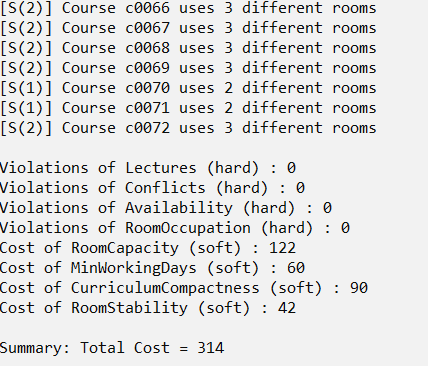
\includegraphics[width=\textwidth]{validator.png} 
    \caption{Validation output showing the detailed list of constraint violations and the total cost.}
    \label{fig:validation_output}
\end{figure}

\paragraph{Evaluation Metrics}\

The output of the validation tool is divided into two parts. The first one provides a very detailed list of any violations encountered that are categorized between hard and soft constraints. Then, the penalty scores associated with these violations, as well as the total cost, are calculated in the summary part. The fitness function used within the MSPSO algorithm is tailored to minimize total cost by meeting hard constraints at first and wherever possible reducing the penalties of the soft constraints.

To highlight the effectiveness of the MSPSO algorithm, its performance is benchmarked against existing methods from the literature. Metrics such as the number of hard constraint violations, the total cost, and the quality of the generated timetables are used for comparison. 


\subsection{Deployment}
\label{subsec:deployment}

\begin{figure}[H]
    \centering
    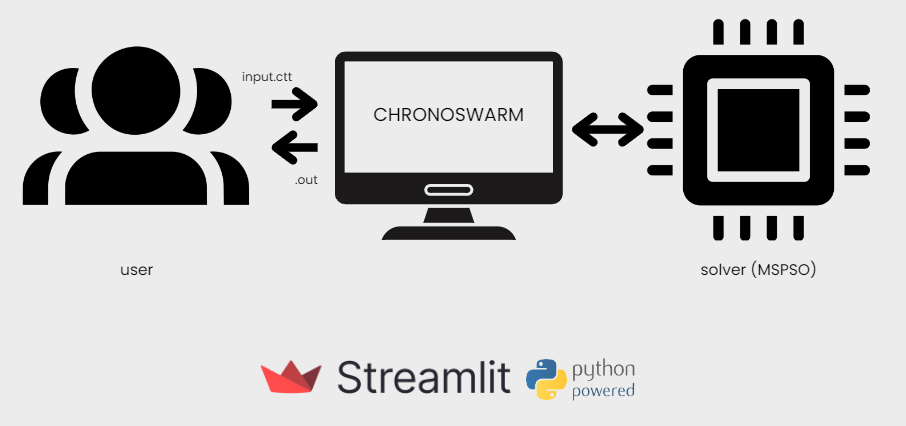
\includegraphics[width=\textwidth]{deployment.png} 
    \caption{Overview of the deployment framework. The user interacts with the system through the ChronoSwarm interface, which communicates with the MSPSO solver to generate and validate optimized schedules.}
    \label{fig:deployment_framework}
\end{figure}

The solution is developed as a web application in the Streamlit Python framework. It presents an interface where users can upload dataset files to run the MSPSO algorithm and automatically generate optimized timetables. The application would output the timetable in a user-friendly format and give an indication of the quality of the solution returned, including constraint violations and overall cost.
